\subsubsection{Color code}
The color code's parity-check-matrix's 
rows are both the code's X stabilizers and Z stabilizers.
Any three-colorable and three-valent graph represents a valid color code.
On the color code, an error is bounded by syndromic faces of all colors.
The simplest color code is the [[7,1,3]] Steane code \cite{steane}. 
\\
\begin{figure}[h!]
	\begin{center}
	\captionsetup{justification=centering,margin=2cm}
	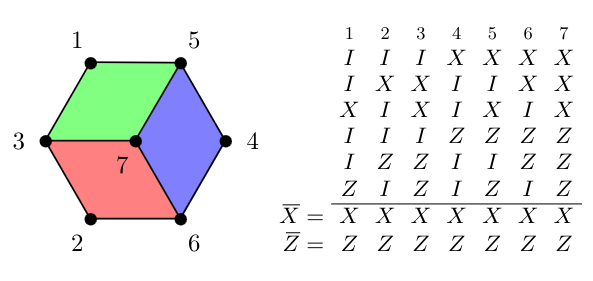
\includegraphics[scale=0.6]{./img/figures/steane.png}\\
	\caption{Graph for the [[7,1,3]] color code, also known as the
    Steane code , and its stabilizers. 
    Figure from \cite{steane}.}
        
	\label{fig: color_graph}
	\end{center}
\end{figure}
% habe ich von erster google bildsuchen seite